\documentclass[letterpaper]{physor2024}

%%% Packages Required by Class (already included)
% fancyhdr
% lastpage
% titling
% titlesec
% ragged2e
% enumitem
% amsmath
% graphicx
% geometry
% newtxtext
% newtxmath
% hyperref
% cleveref
% caption
% authblk
% apptools
% appendix
% ifpdf
% epstopdf

%%% Some other useful packages
% \usepackage{tikz}
% \usepackage{color}
% \usepackage{subcaption}
% \usepackage{algcompatible}
% \usepackage{bm}
% \usepackage{array}

% GLOSSARIES
\usepackage[acronym,nomain,nonumberlist,nogroupskip,nopostdot]{glossaries} % for glossary of acronyms
\setacronymstyle{long-short}
\loadglsentries{glossary}
\makeglossaries
% \renewcommand*{\glstextformat}[1]{\textcolor{black}{#1}} % make glossary color black

% % This file contains custom commands that Lewis uses frequently in LaTeX documents

\usepackage{subcaption}
\usepackage{hyperref}
\hypersetup{colorlinks,allcolors=black}
% % for more https://tex.stackexchange.com/questions/88400/hyperref-changing-the-linkcolor-locally-in-the-toc

% custom equation commands
\newcommand{\QOR}{\qquad \text{OR} \qquad}
\newcommand{\QAND}{\qquad \text{AND} \qquad}
\newcommand{\QTHUS}{\qquad \text{THUS} \qquad}
\newcommand{\QWITH}{\qquad \text{WITH} \qquad}
\newcommand{\QFOR}{\qquad \text{FOR} \qquad}
\newcommand{\QSO}{\qquad \text{SO} \qquad}
\newcommand{\QWHERE}{\qquad \text{WHERE} \qquad}
\newcommand{\QWHEN}{\qquad \text{WHEN} \qquad}
\newcommand{\LINE}{\par\noindent\rule{\textwidth}{0.4pt}\par}
\newcommand{\toinf}{\rightarrow\infty}
\newcommand{\tozero}{\rightarrow0}
\newcommand{\qeq}{\overset{?}{=}}
\newcommand{\ceq}{\overset{\checkmark}{=}}
\newcommand{\Poi}{\text{Poisson}}
\newcommand{\keff}{$k_{e\!f\!f}$}
\newcommand{\kinf}{$k_{\!i\!n\!f}$}
\renewcommand{\epsilon}{\varepsilon} % squiggly epsilon

\def\brac#1{\{#1\}}
\def\Brac#1{\big\{#1\big\}}
\def\BRAC#1{\bigg\{#1\bigg\}}
\def\angbrac#1{\langle#1\rangle}
\def\Angbrac#1{\big\langle#1\big\rangle}
\def\ANGBRAC#1{\bigg\langle#1\bigg\rangle}
\usepackage{float}
\usepackage{multirow} % for special table
% % SI Units
\usepackage{siunitx}
\DeclareSIUnit\n{n}
\DeclareSIUnit\sp{sp}
% \title{OpenMC Depletion Analysis of a TRISO Fueled, Helium Cooled Microreactor}
\title{Exploring Effects of Homogenization on an OpenMC Depletion Analysis of a TRISO Fueled, Helium Cooled Microreactor}

\addAuthor[ligross@wisc.edu]{Lewis I. Gross}{1}
\addAuthor{Patrick Shriwise}{2,1}
\addAuthor{Benjamin Lindley}{1}
\addAuthor{Paul P.~H. Wilson}{1}

%%% Affiliations (from authblk)
%%% \addAffiliation{affiliationNumber}{Name of Institute, City, State/Country}
\addAffiliation{1}{University of Wisconsin - Madison, Madison, Wisconsin}
\addAffiliation{2}{Argonne National Laboratory}

\Abstract{OpenMC is a state-of-the art, open-source Monte Carlo transport code. This work used OpenMC for depletion analysis of an infinite, unit cell model of the Virtual Test Bed gas-cooled microreactor. This microreactor is prismatic, TRISO-fueled, and helium gas cooled. Since the gas-cooled microreactor is intended for load-following, depletion analyses were conducted for 100\%, 50\%, and 10\% of the rated power (225 kW$_{th}$) both for fully explicit and partially explicit TRISO representation, along with a fully homogenized reference case. While a 10\% power is much lower than standard load following contexts, its inclusion offers a low power density comparison. The time steps selected ensure the same total burnup accrues at each depletion step for all power levels. The goal of these analyses is to understand what degree of explicit representation will be necessary for a full-core model. The system eigenvalue, \kinf, was computed as a function of burnup for each representation along with $\Delta \rho$ comparisons between the cases. Xenon-135 and plutonium-241 number densities, which are key factors in explaining the observed \kinf~trends, are included. The $\Delta \rho$ comparisons show that the difference between explicit and kernel only is an order of magnitude better than either of the homogenized reference comparisons between explicit or kernel only. This and similar isotopic trends suggest that a kernel only representation can achieve sufficient accuracy while saving on memory requirements for a full-core model.}

%%% List up to 5 keywords separated by a comma
\keywords{OpenMC, TRISO, depletion, microreactor, gas-cooled}

%%% Provide a short title for the header on odd pages
\shortTitle{Depletion of a TRISO Fueled, Gas-Cooled Microreactor }

%%% Provide a short author listing for the header on even pages
\authorHead{Gross and Wilson}

%%% If LaTeX reports the line number of an error at \begin{document} it
%%%   is most likely due to an error in one of the commands above
\begin{document}

\section{INTRODUCTION}\label{sec:intro}
For advanced reactors, especially those early in the design stage, sufficient \gls{ms} are required to ensure the success of the design concept. Before any system can be built, modelers must prove systems perform safely. The \gls{vtb} \cite{vtb2023} is a repository of reactor models used for research and demonstration of current tools in the nuclear industry as a part of the \gls{neams} initiative. Various types of reactors are available on the \gls{vtb}. Microreactors are one viable class of next generation systems with ongoing modeling efforts using \gls{neams} tools \cite{Stauff-preliminary-applications-2021, Stauff-applications-2022, Abdelhameed-ANS-2022}. One key advantage of microreactors is the ability to supply power to regions with low base load demand or to areas needing temporary power, e.g.~natural disaster relief efforts. There is interest in high-temperature gas microreactors, namely \glspl{gcmr}. Adding the benefits of higher electricity conversion efficiency to a microreactor synergizes with the melting temperature of \gls{triso} fuel, bringing many attractive features together.

Due to the smaller size of microreactors, it is conceivable to move them at some point during operation, e.g. if power was only needed temporarily, or after shutdown but before refueling. In this case, for shielding and criticality safety reasons, the state of the core must be fully understood. If a system has been running on the order of months, the core state has certainly changed from the initial loading.

Previous work on the \gls{vtb} \gls{gcmr} includes analysis of the system for a two day load-following transient \cite{Abdelhameed-ANS-2022}. This work coupled Griffin, BISON, and SAM using the \gls{moose} framework. Griffin computed a solution to the neutron transport equation using a deterministic method, specifically the discrete ordinates and discontinuous finite element methods with coarse mesh finite difference acceleration. BISON is a fuel performance code that computed heat conduction in the solid parts of the system. SAM is a systems analysis code that computed heat transfer in the coolant channels. Since Abdelhameed et al.~only modeled 48 hours, depletion was not considered. Any analysis occurring far enough into an operation cycle requires a burnup simulation to know the state of isotopics in the core, whether computing an accident source term or shielding requirements for transporting the reactor after a shutdown.

A few depletion studies of other microreactor concepts exist. A study of the gas-cooled, Japanese \gls{httr} computed criticality and burnup using various cross section representations with SCALE6 and MCNP5/X \cite{chiang-gcmr}. Another study looked at burnup for Westinghouse's eVinci \gls{hpmr}, finding that it could operate for at least 10 years without refueling as a nuclear battery \cite{Hernandez-hpmr}. This work adds the first depletion analysis to the \gls{vtb} \gls{gcmr}.

While \gls{triso} is expected to have favorable fuel performance in advanced reactors \cite{triso-overview}, it poses significant modeling challenges, especially in Monte Carlo, due to the high number of surfaces per reactor. Many advanced reactors that use \gls{triso} will need to find ways to perform high-fidelity \gls{ms} with this limitation. Homogenization is one way of handling the memory requirement of \gls{triso} simulations, but full fuel homogenization is known to be unreliable. The differences in eigenvalue come from slowing down of neutrons, specifically which materials they interact with as they thermalize and attempt to cause new fissions. A fully explicit \gls{triso} has layers of \gls{pyc} and silicon carbide surrounding the kernel. When \gls{triso} is fully homogenized, neutrons have fewer chances to thermalize before interacting with fuel atoms, and thus are more likely to be absorbed in a resonance. However, the slowing down of neutrons in background graphite is expected to be similar to slowing down in the non-fuel \gls{triso} components. This motivates a partial homogenization approach with the goal of balancing simulation memory requirements with simulation accuracy.

A partial homogenization, herein named ``kernel only," homogenizes all non-fuel \gls{triso} layers into the background of the fuel compact. This gives spherical fuel kernels packed into graphite doped with \gls{pyc} and silicon carbide. Despite known inaccuracies of fully homogenized compacts, this work quantifies the difference in the eigenvalue for the \gls{gcmr} as a basis for what kind of representation must be included in a full-core model. In order to gain understanding of how the kernel only case performs compared to fully explicit, the fully homogenized case must be included as a reference.

Previous work for the \gls{vtb} \gls{gcmr} used Griffin for neutron transport, however, this work chose OpenMC for a few reasons. First, OpenMC is an \gls{oss}; the code is free to use for verification. As a Monte Carlo code, there are advantages over a deterministic code, like Griffin, for depletion analysis. The microscopic cross sections are more accurate in continuous energy format when modeling the resonance region, as opposed to representing them with multi-group cross sections. OpenMC tallies reaction rates--or flux--directly from continuous energy cross sections, avoiding the need to do fine and coarse-group simulations to appropriately handle system heterogeneity. The reaction rates are then used for depletion.

The rest of this paper will be organized as follows. \cref{sec:depletion} will provide some background theory on depletion. \cref{sec:openmc_model}  will detail the \gls{vtb} \gls{gcmr} and its components, explaining the OpenMC model and the depletion schemes. \cref{sec:results} will present results for the system. \cref{sec:conclusions} will interpret those results and discuss the plans forward for more \gls{ms}.

\section{DEPLETION THEORY}\label{sec:depletion}
% Once any reactor starts running, the composition of isotopes will change over time. Nuclides exposed to neutron flux will transmute into radioisotopes that have various modes of decay, creating new isotopes that did not exist at the start of operation, as well as decaying into other isotopes already in the system. The rate at which isotopes transmute and decay into each other depends on the transport solution via the reaction rates, which depend directly on the neutron flux. This relationship causes the coupling between transport and depletion to behave non-linearly \cite{romano-depletion-2021}.

% Certain isotopes have more influence on the system than others. For example, xenon-135 has an extremely high neutron absorption cross section, to the point that it influences the positioning of the control elements. Xenon-135 is important in load-following contexts, in which the power changes once or twice per day, as its concentration increases when power decreases, and it is burned off when power increases again. This matters more in load-following mode because the xenon-135 half-life is on the order of 9 hours \cite{d-and-h}. For context, the load following schedule in Abdelhameed et al. has high power for 12 hours, low power for 7 hours, and 2.5 hour ramps between, inspired from the NEA OECD report on load-following \cite{Abdelhameed-ANS-2022,nea-oecd-LF}.

To model burnup, transmutation and decay cross sections of the isotopes are combined with the flux to determine production and destruction rates for each isotope. These formulate a system of differential equations for the nuclide densities. For isotope $i$ with number density $N_{i}(t)$, the Bateman or burnup equations describe the time dependent isotopic composition, given by
\vspace*{-0.1cm}
\begin{multline} \label{eq:batemen}
    \frac{dN_{i}}{dt} =
    \sum_{j} \bigg[\int_{0}^{\infty} \sigma_{j\rightarrow{i}}(E,t)\phi(E,t)dE + \lambda_{j\rightarrow{i}}\bigg]N_{j}(t) \\
    -\bigg[\int_{0}^{\infty} \sigma_{i}(E,t)\phi(E,t)dE
    +\sum_{j}\lambda_{i\rightarrow{j}}\bigg] N_{i}(t),
\end{multline}

\noindent where $\sigma_{j\rightarrow{i}}(E,t)$ is the transmutation cross section of isotope $j$ that produces isotope $i$ at energy $E$ at time $t$, and $\lambda_{j\rightarrow{i}}$ are the decay constants for decay modes in nuclide $j$ that produce nuclide $i$. The system of equations for isotopes $i\in[1,n]$ can be expressed in matrix notation using the nuclide vector $\mathbf{n}\in\mathbb{R}^{n}$
\begin{equation} \label{eq:burnup matrix odes}
    \frac{d\textbf{n}}{dt} =
    \textbf{A}(\textbf{n},t) \textbf{n}
    \QWITH
    \textbf{n}(0) = \textbf{n}_{0},
\end{equation}

\noindent where $\textbf{A}\in\mathbb{R}^{n\times n}$ is the burnup matrix. Since the transport equation depends on number density and $\textbf{A}$ depends on the solution to the transport equation, $\textbf{A}$ then also depends on number density. Because ``the timescale over which material compositions change is sufficiently long ... the transport equation can be solved as a steady-state equation" \cite{romano-depletion-2021}. Taking the burnup equations as quasi steady-state allows the earlier non-separable equation to be solved via separation solution
\begin{equation} \label{eq:separable burnup matrix odes}
    \frac{d\textbf{n}}{dt} =
    \textbf{A}(\textbf{n}) \textbf{n}
    \QWITH
    \textbf{n}(0) = \textbf{n}_{0},
\end{equation}

\noindent The solution to which is
\begin{equation} \label{eq:separation solution}
     \textbf{n}(t) = e^{\textbf{A}t} \textbf{n}_{0}
\end{equation}

\noindent Solving \cref{eq:separable burnup matrix odes} numerically involves two separate components \cite{romano-depletion-2021}:
\begin{enumerate}
    \item Using a numerical method to integrate the matrix $\textbf{A}$ in \cref{eq:separable burnup matrix odes} forward in time. This usually involves taking one or more matrix exponential.
    \item Evaluating the matrix exponential $\exp(\textbf{A}t)$ or the action of the matrix exponential on a vector of nuclide concentrations.
\end{enumerate}

OpenMC provides all the software infrastructure necessary to compute a burnup simulation, thus users only need to define a model. The next section will discuss the OpenMC model.

\section{OPENMC MODEL}\label{sec:openmc_model}
This section will describe the \gls{gcmr} system and its OpenMC model. \cref{sec:system} explains the system specifications and geometric parameters of the \gls{gcmr}. \cref{sec:model_def} explains the OpenMC model and its important components for depletion. Finally, \cref{sec:depl_sim} outlines the depletion simulation settings.

\subsection{System Description}\label{sec:system}
\cref{fig:vtb_gcmr} shows a diagram of the \gls{gcmr}. Graphite is the structural material holding the cylindrical compacts arranged in a hexagonal lattice. \cref{tab:dimensions} shows various system parameters. The fuel compacts contain \gls{triso} spheres packed into graphite. The moderator uses YH$_{2}$ with a thin Cr coating encased in a FeCrAl envelope; the coating is between the YH$_{2}$ and the envelope. The poison compacts contain burnable B$_{4}$C spheres packed into graphite. The coolant is helium. The upper and lower reflectors are BeO. Since the goal of this work is to determine excess reactivity, the B$_{4}$C control rod is not inserted into the active core region and stays in the upper reflector. The central compact in the core is instead filled with non-circulating helium \cite{Abdelhameed-ANS-2022}. A cosine heating distribution was used to approximate temperature: inlet $T=873.15$ K, outlet $T=1133.65$ K. The lower reflector was set to the inlet temperature and the upper reflector was set to the outlet temperature.
\vspace*{-0.2cm}
 \begin{figure}[h]
    \centering
    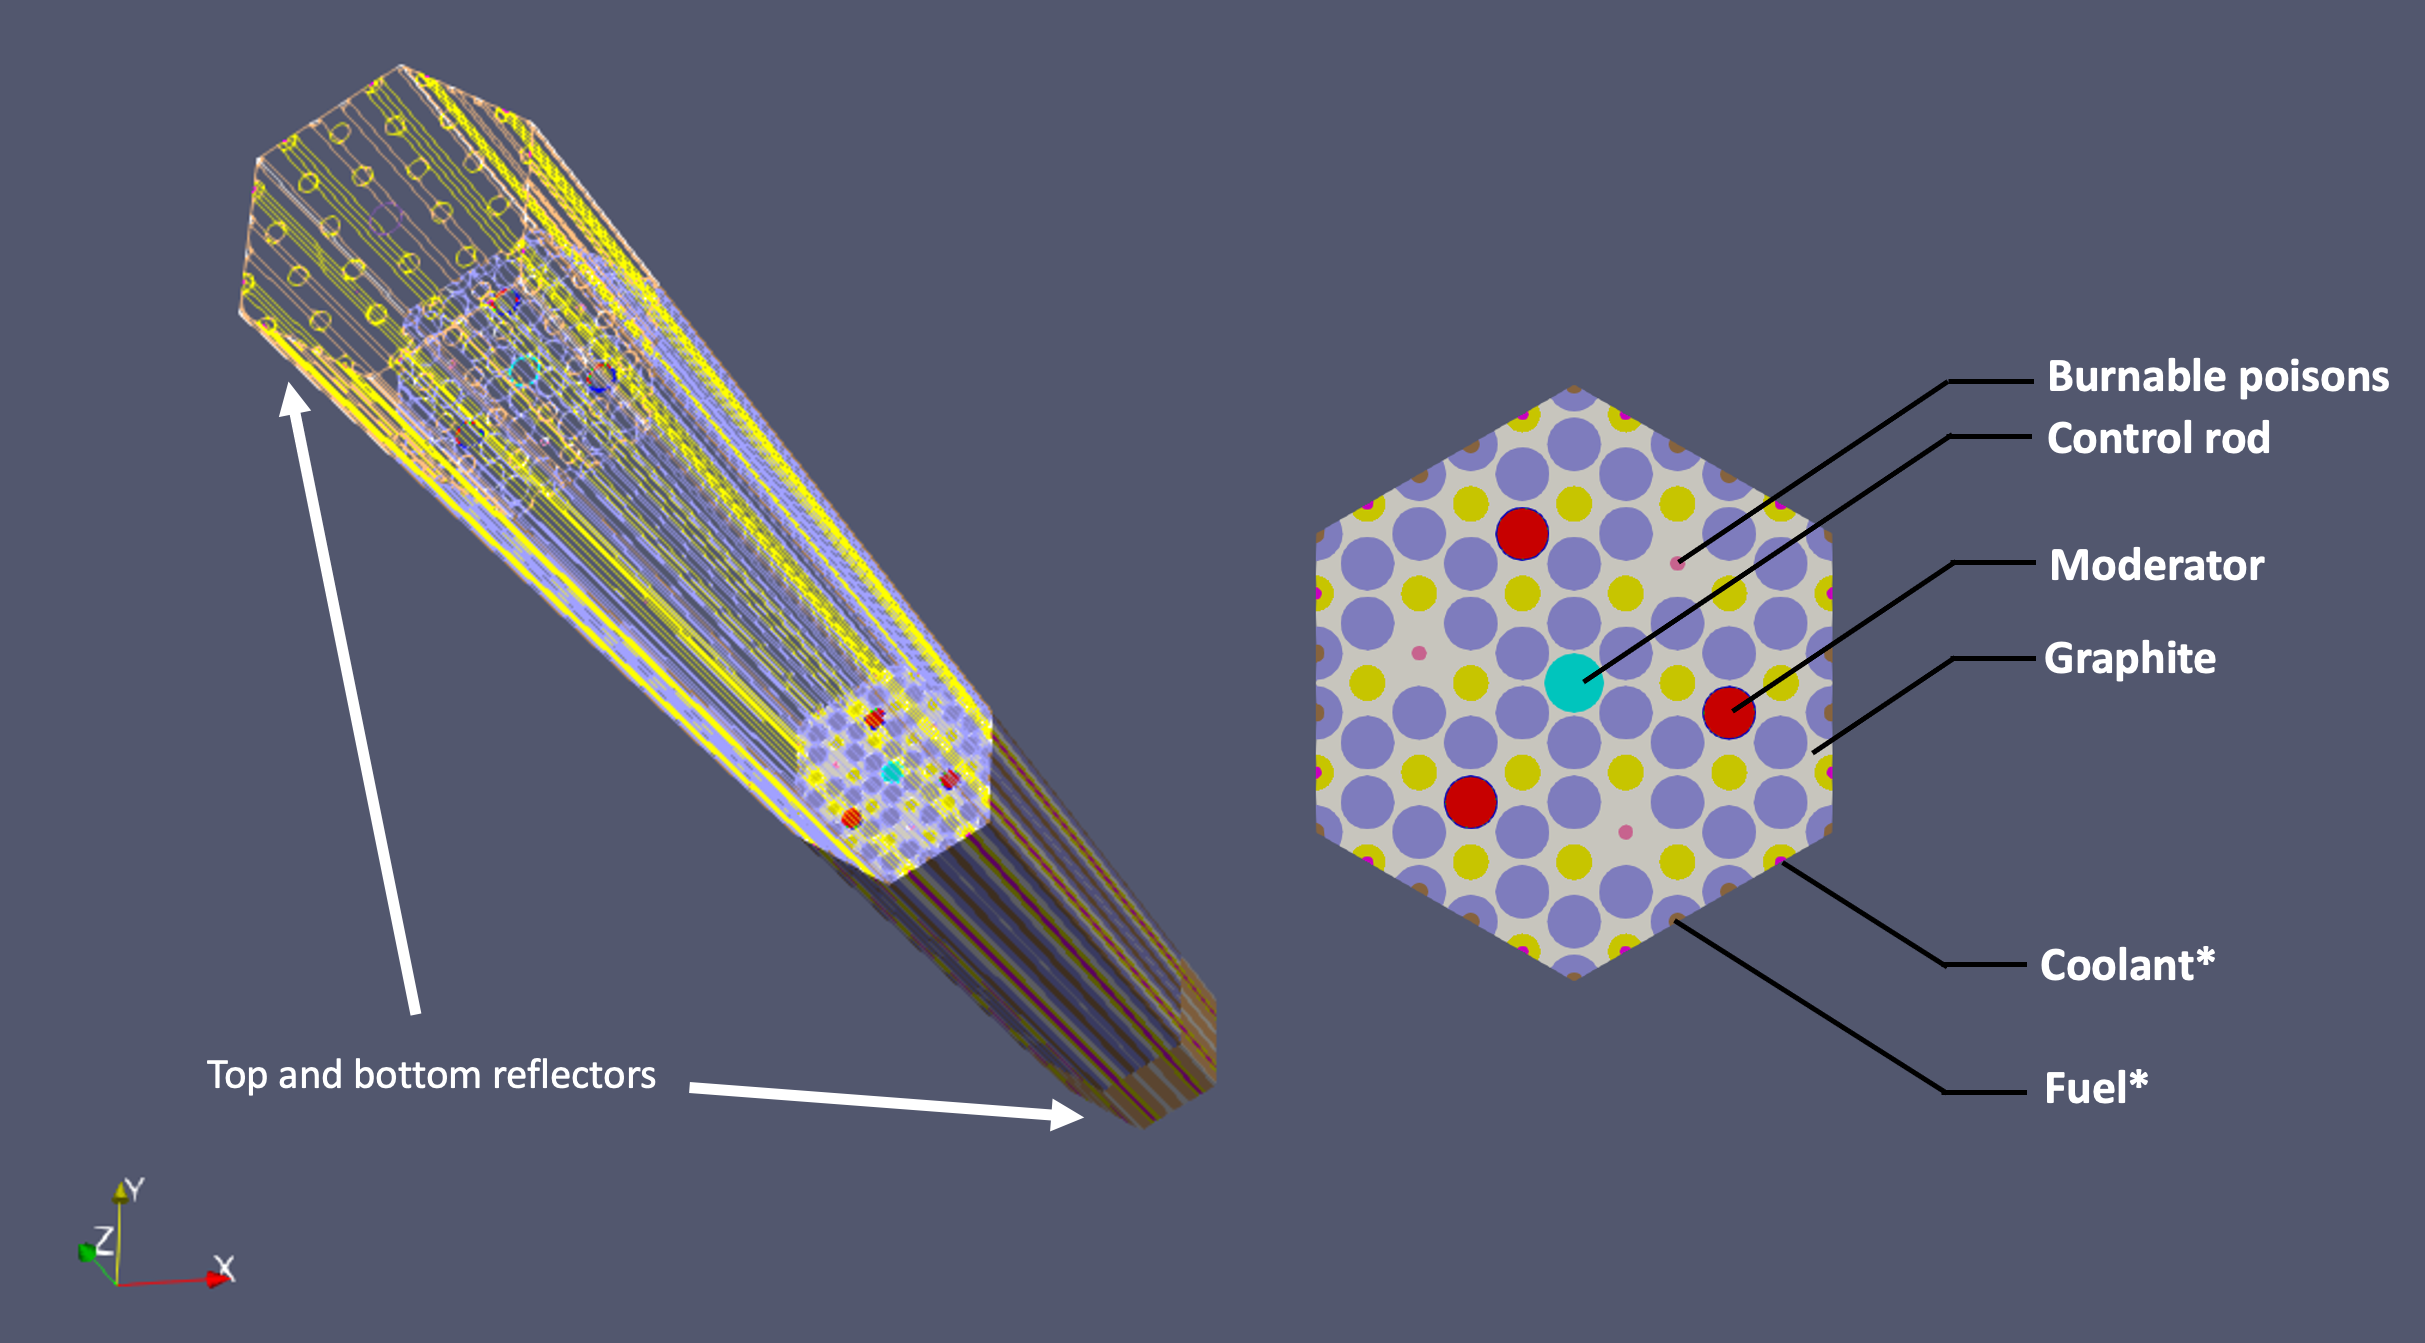
\includegraphics[width=0.625\linewidth]{figures/vtb_gcmr_diagram.jpg}
    \caption{The above visualization shows the \gls{vtb} \gls{gcmr} unit cell: both a cross section of the fuel region and a 3D rendering of the fuel and reflectors \cite{Stauff-applications-2022}.}
    \label{fig:vtb_gcmr}
\end{figure}
\vspace*{-0.5cm}
\begin{table}[h]
    \centering
    \caption{This table summarizes key dimensions (radii, thicknesses) of the compacts and parameters of the fuel and poison.}
    \begin{tabular}{|c|c|c|c|c|c|}
    \hline
    fuel radius & poison radius & moderator radius, Cr coating & control radius & coolant radius \\
    0.90 cm & 0.25 cm   & 0.843 cm, 0.007 cm & 0.99 cm    & 0.60 cm  \\
    \hline
    FeCrAl thickness & pin pitch & fuel packing fraction & poison packing fraction & enrichment \\
    0.05 cm & 2.00 cm  & 0.4 -  & 0.25 - & 19.95\% \\
    \hline
    \end{tabular}
    \vspace{-0.5cm}
    \label{tab:dimensions}
\end{table}

\subsection{Model Definition}\label{sec:model_def}
The system is divided into axial layers to allow for spatial variation in depletion. While Abdelhameed et al. chose two axial layers per reflector and 16 layers in the active region \cite{Abdelhameed-ANS-2022}, due to memory constraints, all cases in this study used eight layers in the active region. The reflectors are 20 cm high and the core is 160 cm high. Within each layer there is 3-way symmetry, which can be seen by slicing the hexagon in \cref{fig:core_slice_sbs} into any three 120 degree sectors. To take advantage of this, fuel compacts are depleted identically to their two sister compacts at the corresponding symmetry points, yielding 18 unique depletable fuel regions per layer. Additionally, to allow the B$_{4}$C to burn, poison compacts add a 19th depletable region per layer. \cref{fig:core_slice_sbs} shows a radial slice of the fuel portion of the reactor. \cref{fig:reflectors} shows a radial slice of each reflector region. The only difference between the explicit, kernel only, and homogenized cases is the fuel representation. The distribution of fuel kernels is the same between the fully explicit and kernel only, they only differ in what material is outside the kernels.

\begin{figure}[!h]
    \centering
    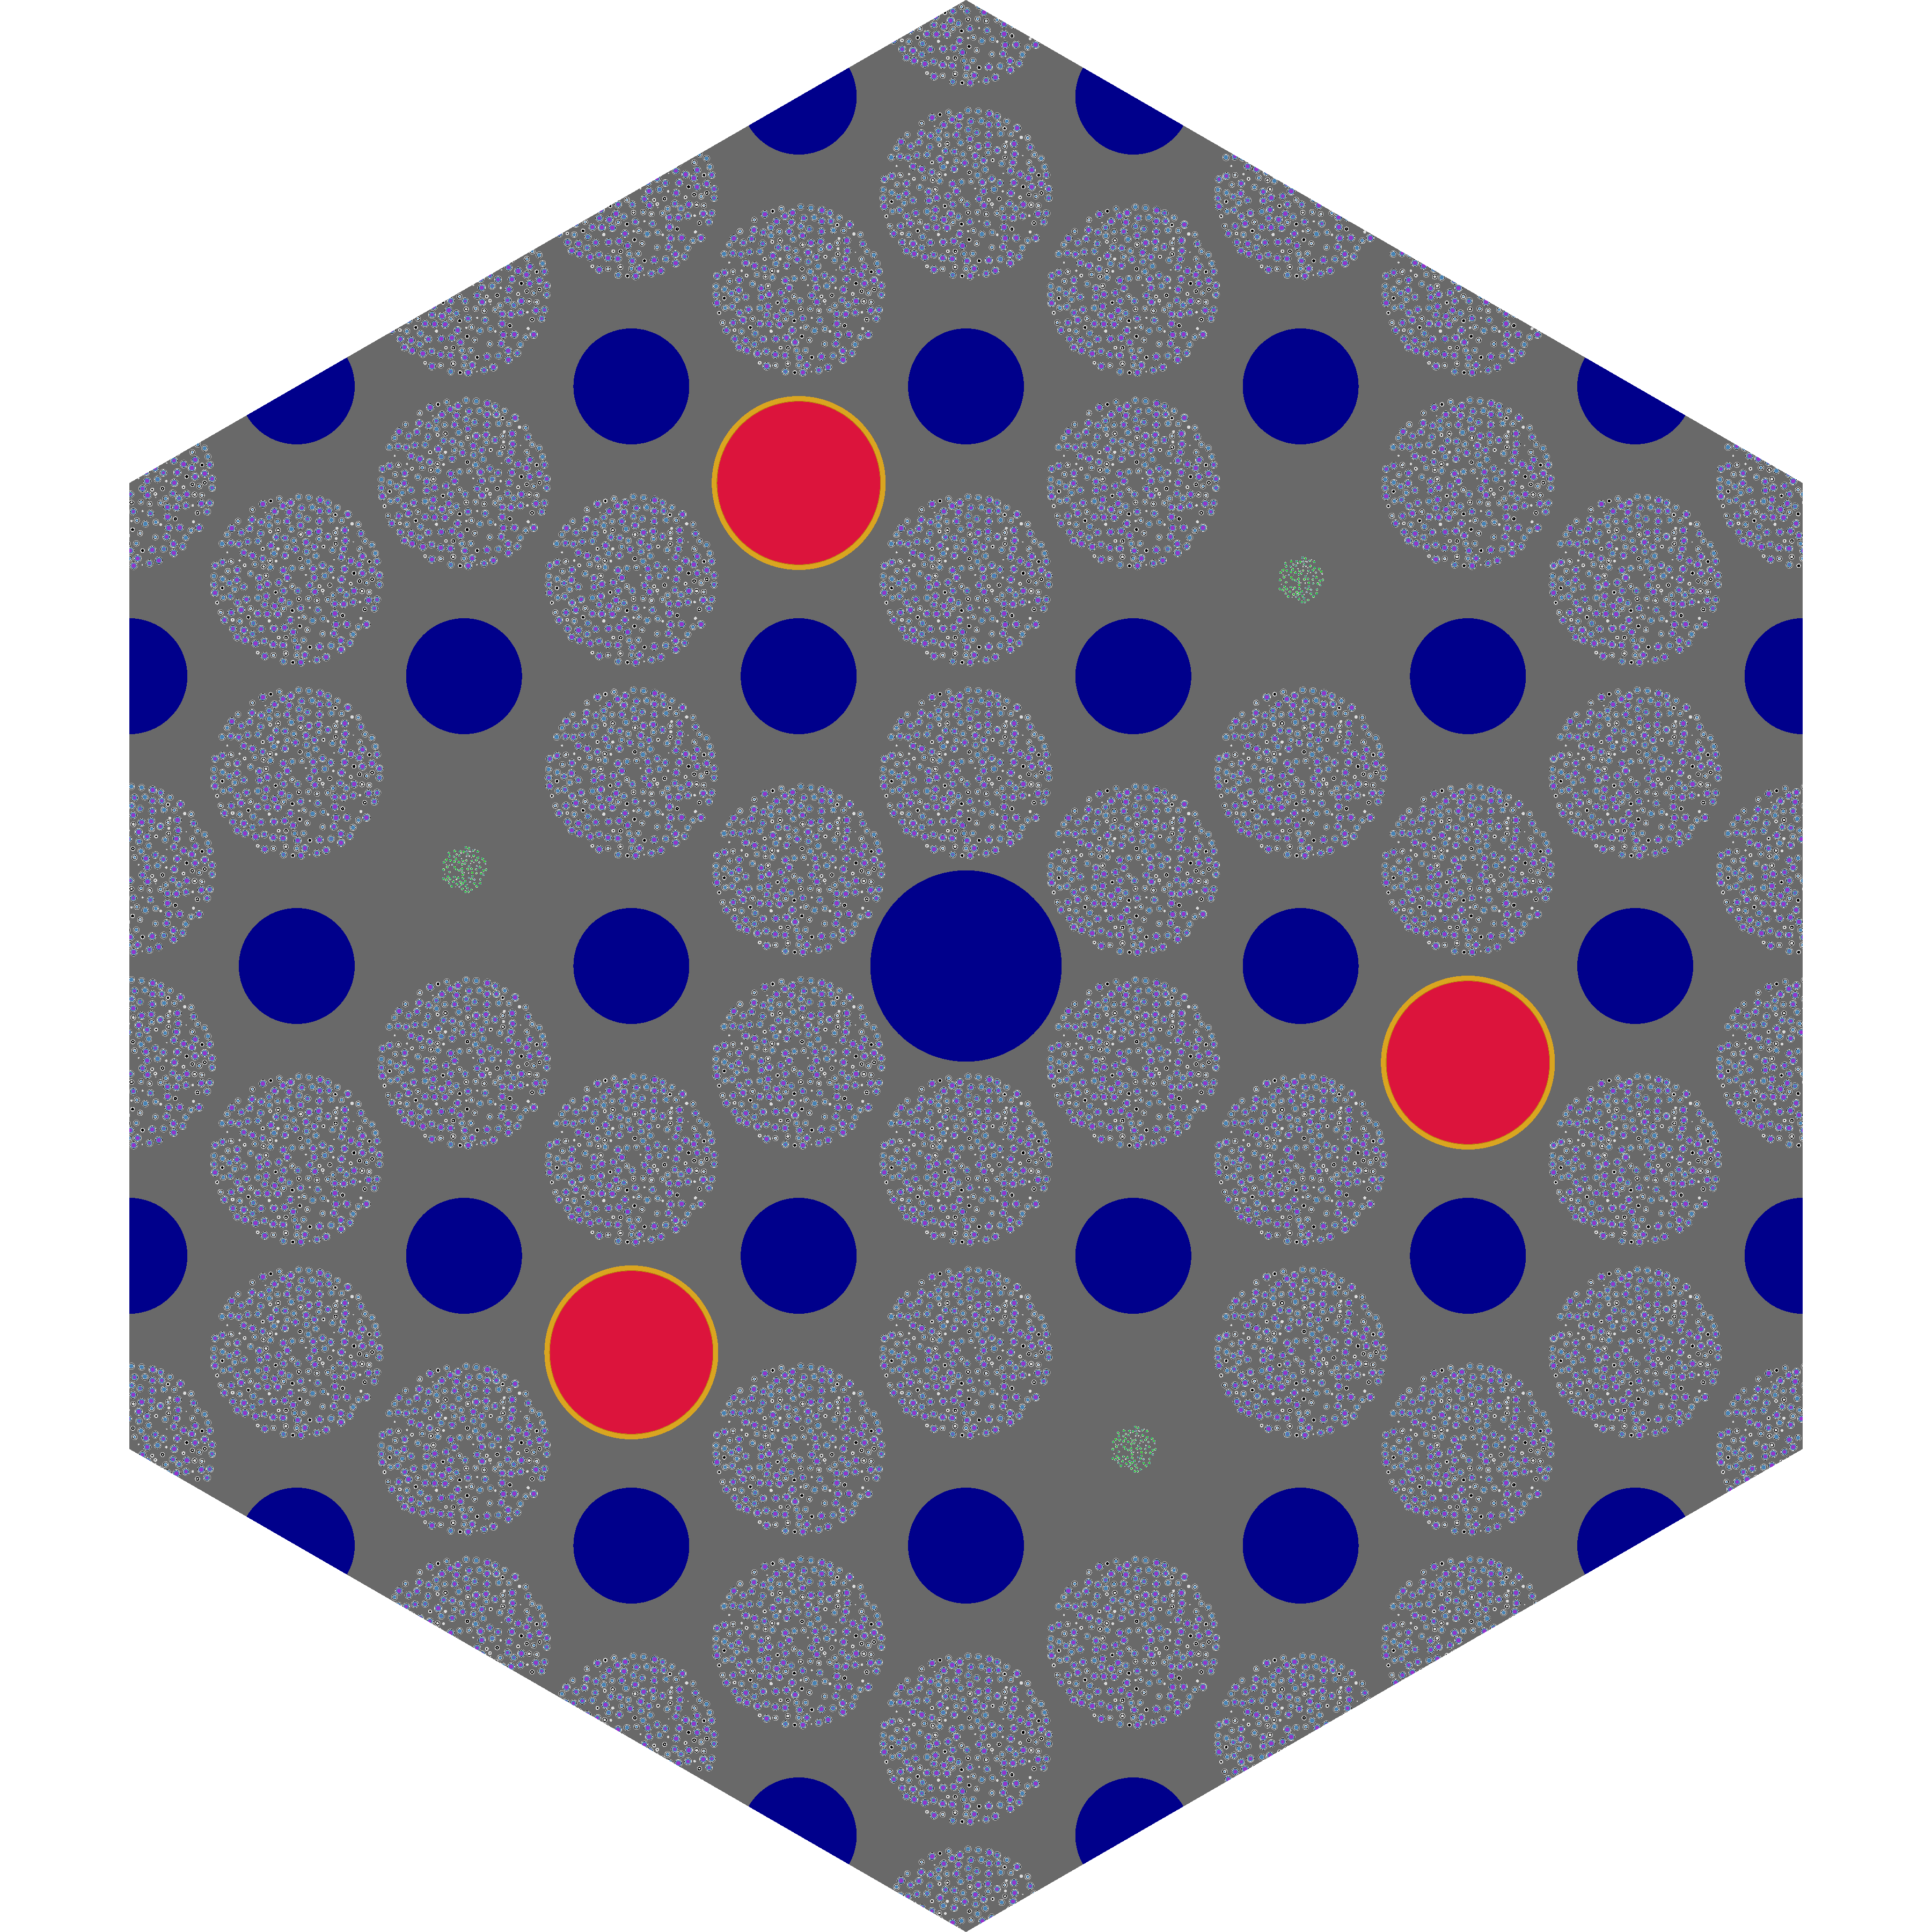
\includegraphics[width=0.325\linewidth]{figures/active_height.png}
    \label{fig:active_slice}
    \caption{This figure shows a radial slice of the active region. Gray corresponds to graphite in the matrix or pyrolitic carbon, dark blue corresponds to helium coolant, red corresponds to YH$_{2}$ moderator, gold corresponds to FeCrAl, green corresponds to the B$_{4}$C poison particles (packed at 25 percent in graphite), and purple corresponds to the fuel kernel in the \gls{triso} particles (packed at 40 percent in graphite).}
    \label{fig:core_slice_sbs}
\end{figure}
\begin{figure}[!h]
    \centering
    \begin{subfigure}{0.475\linewidth}
        \centering
        
\includegraphics[width=0.6\linewidth]{figures/lower_reflector.png}
        \caption{A slice of the lower reflector, colored by material.}
        \label{fig:lower_reflector_slice}
    \end{subfigure}
    \begin{subfigure}{0.475\linewidth}
        \centering
        
\includegraphics[width=0.6\linewidth]{figures/upper_reflector.png}
        \caption{A slice of the upper reflector, colored by material.}
        \label{fig:upper_reflector_slice}
    \end{subfigure}
    \caption{This figure shows a  radial slice of the lower reflector (left) and the upper reflector (right). The difference between the upper and lower reflectors is that the upper reflector has an extra compact for the B$_{4}$C control rod. Dark blue corresponds to helium coolant and light blue corresponds to BeO, while the B$_{4}$C control rod is shown in green.}
    \label{fig:reflectors}
    \vspace*{-0.4cm}
\end{figure}

\subsection{Depletion Simulation Definition}\label{sec:depl_sim}
With complete geometry and material definitions, the depletion simulation defines power history, time steps, and an integration scheme. OpenMC then alternates between transport and Batemen equation solves. The eigenvalue simulations used 25 inactive batches and 75 active batches with 10000 particles per batch. The cross sections used for transport are continuous energy from ENDF-B-VII.1. The chain file, an XML file used for depletion in OpenMC, contains transmutation and decay data necessary to compute the burnup matrix. This simulation used a chain based on the \gls{casl} project \cite{CASL-report} and is provided by OpenMC \cite{openmc-chains}. While the chain originates from a \gls{lwr} system, the similarity of the neutron spectrum, i.e. both thermal, makes this chain file a good choice, since $\phi(E)$ is one of the inputs when computing the burnup matrix. The \gls{casl} chain can be found on OpenMC's website, specifically the portion that provides data for users to download.

Predictor-Corrector methods are commonly used for time integration in burnup contexts. In this study, the second order \gls{cecm} is chosen, which OpenMC implemented based on work comparing various integration schemes for depletion \cite{isotalo_comparison_2015}. Since the method is second order, it requires two transport solves per depletion time step: one for the prediction and one for the correction.

In order to uphold the quasi-static burnup assumption, it is important to use fine time steps when nuclide concentrations are expected to be changing rapidly. In reactor contexts, this occurs at the beginning of the simulation when strong, fission-product poisons, such as xenon and samarium, jump from zero to an equilibrium concentration. The time steps can be lengthened after the initial transient behavior reaches a steady-state. For all full power cases, the time steps used: five one-day time steps, three five-day time steps, three fifteen-day time steps, and 25 60-day time steps. In order to keep the burnup the same at each step for all other powers, the half and tenth power cases use the same number of steps, with twice and ten times as long steps, respectively.

\section{RESULTS}\label{sec:results}
In this section, the eigenvalues will be compared between the varying fuel representations as a function of burnup. \cref{fig:kinf_full_explicit_results} shows \kinf~vs burnup with $2\sigma$ statistical error bars for the fully explicit case as a representative. \cref{fig:pcm_diffs} shows comparisons between all cases via reactivity difference, $\Delta \rho$ in units of \gls{pcm}, with propagated $2\sigma$ statistical error bars. If the first set of eigenvalues is $k_ 1$ and the second set is  $k_2$, $\Delta \rho$ is defined
\begin{equation}
    \Delta \rho \equiv
    \rho_1 - \rho_2 =
    \frac{k_1-1}{k_1} - \frac{k_2 - 1 }{k_2} =
    \frac{1}{k_2} - \frac{1}{k_1}
\end{equation}
\vspace{-0.4cm}
\begin{figure}[!h]
    \centering
    \begin{subfigure}{0.6\linewidth}
        \centering
        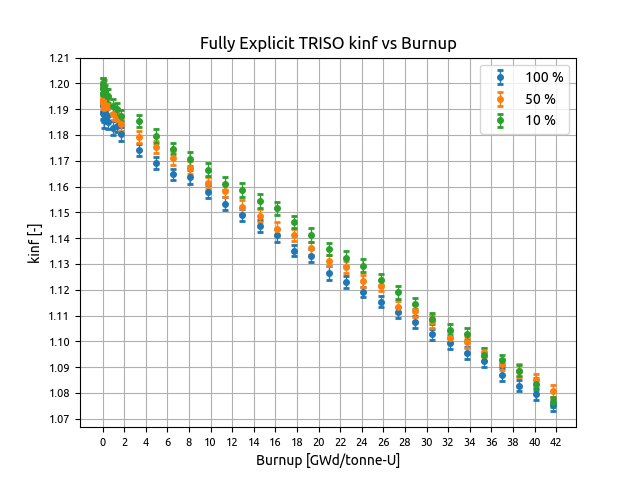
\includegraphics[width=\linewidth]{figures/expl_kinf_vs_bu.png}
    \end{subfigure}
    \caption{This figure shows \kinf versus burnup for the fully explicit case with $2\sigma$ error bars up to $\sim$42 GWd/tonne-U.}
    \label{fig:kinf_full_explicit_results}
\end{figure}

\begin{figure}[!h]
    \centering
    \begin{subfigure}{0.495\linewidth}
        \centering
        \includegraphics[width=\linewidth]{figures/explicit_minus_homog.png}
        \caption{Explicit minus homogenized}
    \end{subfigure}
    \begin{subfigure}{0.495\linewidth}
        \centering
        \includegraphics[width=\linewidth]{figures/kern_minus_homog.png}
        \caption{Kernel only minus homogenized}
    \end{subfigure}
    \begin{subfigure}{0.495\linewidth}
        \centering
        \includegraphics[width=\linewidth]{figures/explicit_minus_kern.png}
        \caption{Explicit minus kernel only}
    \end{subfigure}
    \caption{This figure shows the $\Delta \rho$ versus burnup with $2\sigma$ error bars on \kinf for the pairs of each representation up to a burnup of $\sim$42 GWd/tonne-U.}
    % \vspace*{-0.3cm}
    \label{fig:pcm_diffs}
\end{figure}

\cref{tab:begin_to_end} shows \gls{boc} and \gls{eoc} eigenvalues for each case and power. In \cref{fig:pcm_diffs}, the majority of confidence intervals are overlapping, which seems to indicate that the difference in eigenvalue is weakly, if at all, a function of burnup. In order to compare the scales of the $\Delta \rho$ with one representative number, \cref{tab:average_pcms} shows the average over all $\Delta \rho$ for each difference at each power.

\begin{table}[!h]
    \centering
    \caption{This table shows the \gls{boc} and \gls{eoc} eigenvalues for each representation and power.}
    \begin{tabular}{c|c|c|c|c|}
    \multicolumn{1}{l|}{power} & \multicolumn{1}{c|}{representation} & \multicolumn{1}{c|}{explicit} & \multicolumn{1}{c|}{kernel only} & \multicolumn{1}{c|}{homogenized} \\
    \hline
    \multirow{2}{*}{100\%} & BOC & $1.19995 \pm 0.00218$ & $1.20229 \pm 0.00262$ & $1.17285 \pm 0.00229 $ \\
    \cline{2-5}
     & EOC & $1.07539 \pm 0.00223$ & $1.07855 \pm 0.00247$ & $1.04950 \pm 0.00200 $ \\
    \hline
    \multirow{2}{*}{50\%} & BOC & $1.19995 \pm 0.00218$ & $1.20229 \pm 0.00262$ & $1.17285 \pm 0.00229$ \\
    \cline{2-5}
     & EOC & $1.08086 \pm 0.00231$ & $1.08568 \pm 0.00235$ & $1.05397 \pm 0.00214$ \\
     \hline
    \multirow{2}{*}{10\%} & BOC & $1.19995 \pm 0.00218$ & $1.20229 \pm 0.00262$ & $1.17285 \pm 0.00229$ \\
    \cline{2-5}
     & EOC & $1.07661 \pm 0.00193$ & $1.08328 \pm  0.00245$ & $1.05101 \pm 0.00217$ \\
    \cline{1-5}
    \end{tabular}
    \label{tab:begin_to_end}
    \vspace*{-0.3cm}
\end{table}

\begin{table}[!h]
    \caption{This table shows the average $\Delta \rho$ for each comparison at every power with $2\sigma$ uncertainty.}
    \begin{tabular}{c|c|c|c}
    $\overline{\Delta \rho}$ & explicit - homogenized & kernel only - homogenized & explicit - kernel only \\ \hline
    100\% power & 1966 $\pm$ 49 pcm & 2172 $\pm$ 49 pcm & -206 $\pm$ 48 pcm \\
    50\% power & 1943 $\pm$ 49 pcm & 2184 $\pm$ 49 pcm & -241 $\pm$ 49 pcm\\
    10\% power & 1938 $\pm$ 49 pcm & 2160 $\pm$ 49 pcm & -222 $\pm$ 49 pcm
    \end{tabular}
    \label{tab:average_pcms}
\end{table}

The overall trend is that higher power results in less excess reactivity, despite each depletion step using the same total burnup. Though, the difference between the power levels diminishes as burnup increases, which can be seen in \cref{fig:kinf_full_explicit_results}. Over 34 GWd/tonne-U, all three power levels \kinf are more or less overlapping when considering a $2\sigma$ confidence interval. Both xenon-135 atom densities, shown in \cref{tab:xenons}, and plutonium-241 atom densities, shown in \cref{fig:plutoniums}, are needed to explain this behavior.

\begin{table}[!h]
    \centering
    \caption{This table shows the equilibrium xenon-135 number density from a fuel compact in the middle layer in the innermost ring. All units are atom per cubic centimeter. Since the first five time steps are used to converge xenon, the numbers below are the average of the fifth to the last value for xenon number density.}
    \begin{tabular}{c|c|c|c|}
     representation & explicit & kernel only & homogenized \\ \hline
    100\% power & $2.4176\times 10^{16}$ & $2.4088\times 10^{16}$ & $1.2127\times 10^{15}$ \\  \hline
    50\% power & $1.3395\times 10^{16}$ & $1.3359\times 10^{16}$ & $6.7200\times 10^{14}$ \\ \hline
    10\% power & $2.9367\times 10^{15}$ & $2.9275\times 10^{15}$ & $1.4744\times 10^{14}$ \\ \hline
    \end{tabular}
    \label{tab:xenons}
\end{table}

\begin{figure}[!h]
    \centering
    \begin{subfigure}{0.495\linewidth}
        \centering
        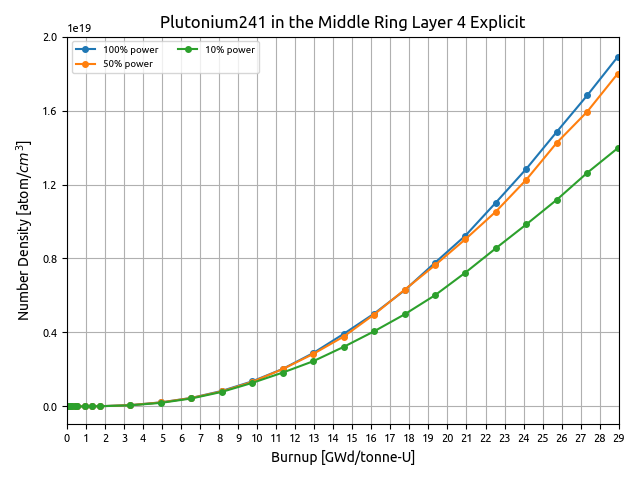
\includegraphics[width=\linewidth]{figures/explicit_Pu_241.png}
    \end{subfigure}
    \begin{subfigure}{0.495\linewidth}
        \centering
        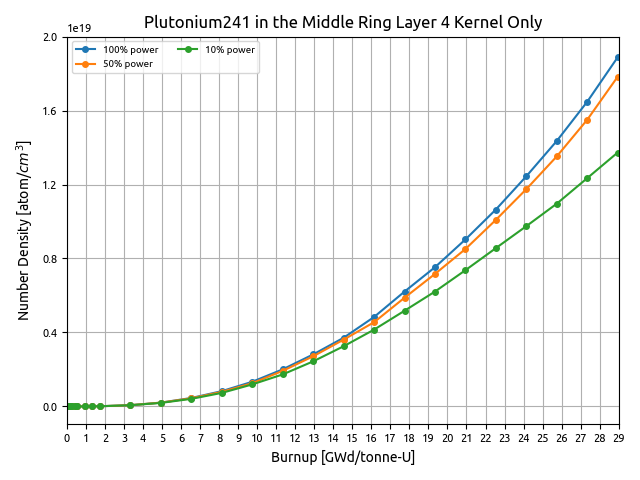
\includegraphics[width=\linewidth]{figures/kernel_only_Pu_241.png}
    \end{subfigure}
    \begin{subfigure}{0.495\linewidth}
        \centering
        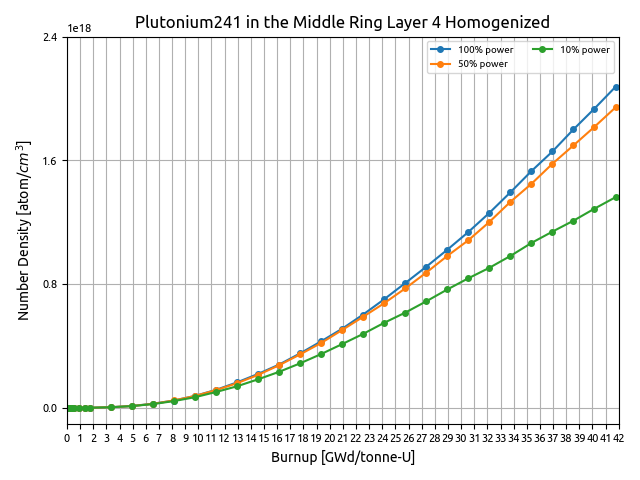
\includegraphics[width=\linewidth]{figures/homogenized_Pu_241.png}
    \end{subfigure}
    \caption{This figure shows plutonium-241 number density from a fuel compact in the middle layer in the innermost ring up to $\sim$42 GWd/tonne-U for each representation.}
    \label{fig:plutoniums}
\end{figure}

In every case, xenon-135 concentration reach an equilibrium level quickly. The higher the power, the higher the equilibrium xenon concentration, meaning more competition with fuel for absorptions. This explains the initial trend that higher power has less excess reactivity, since the negative xenon insertions are larger, despite the same total burnup. Over time, the eigenvalues at each power level start to overlap. At high burnup, xenon is not changing in time, so this cannot explain the high burnup behavior. However, \cref{fig:plutoniums} shows that as burnup increases, each power level's plutonium-241 response differs. In this case, higher power breeds more plutonium. Since plutonium-241 is inserting positive reactivity, the 100\% case, which before had a lower \kinf now starts to gain reactivity. Conversely, the 10\% which previously has the most excess reactivity, starts to lose out on the plutonium insertion compared to the other two powers. This explains why the eigenvalues start to approach each other, since the positive and negative insertions begin to balance.

\section{CONCLUSIONS}\label{sec:conclusions}
This paper simulated an infinite, unit cell model of the \gls{vtb} \gls{gcmr} using the OpenMC Monte Carlo code, adding the first depletion analysis for this reactor. Since the reactor is intended to load follow, it depleted the system at $100\%$, $50\%$ and $10\%$ power. The depletion simulations showed that the reactor still has excess reactivity to at least 42 GWd/tonne-U and likely could extend to upwards of 50 GWd/tonne-U.

This work aims to assess a kernel only representation versus fully explicit \gls{triso} representation. The kernel only representation alleviates memory consumption, which will become more of a limiting factor for a full-core model. The $\Delta \rho$ between fully explicit and kernel only -- ranging from $206\pm48$ \gls{pcm} to $241\pm49$ \gls{pcm} -- was about an order of magnitude better than either case's comparison with the homogenized reference. This is a little high, though not too far off from the computational 100 \gls{pcm} benchmark. Additionally, equilibrium xenon values and plutonium-241 behavior agree decently well for the explicit and kernel only case. These suggest that a kernel only model will be worth pursuing for a full-core model.

Future work includes modeling depletion during repeated load following transients and in a critical configuration to verify the same conclusions. While standalone depletion is a first step in understanding the \gls{gcmr}, but it is of interest to couple depletion into a multiphysics algorithm to aim for as high fidelity simulations as possible. Future multiphysics analyses will rely on Cardinal \cite{novak2022-cardinal}. The Cardinal simulation will couple OpenMC for neutron transport, \gls{moose}'s \gls{htm} for heat conduction, and \gls{thm} for 1-D thermal hydraulics. After verification of standalone simulations, it will be of interest to quantify the impact of depletion on high-fidelity multiphysics.

\section*{ACKNOWLEDGEMENTS}
The authors would like to thank the OpenMC development team for their guidance and assistance with software, as well as the Center for High Throughput Computing at the University of Wisconsin - Madison for their support in using the High Performance Cluster. The first author was supported in part by the US Nuclear Regulatory Commission's Graduate Fellowship Program administered by the University of Wisconsin-Madison.

% \printglossaries

\bibliographystyle{physor2024}
\bibliography{physor2024}

\end{document}